\section{Pregunta 2: Snap roll de un quadcóptero}
\label{sec:p2}

\subsection{Descripción del problema}
Se traslada un quadcóptero desde $\bp_0=(0,0,1)$\,m hasta $\bp_f=(4,2,1.3)$\,m atravesando el agujero de una pared mientras está invertido. Para ello ejecuta un \textit{snap roll}, respetando límites de actuación e inclinación y terminando en reposo con yaw final de $90^\circ$. Se eligió este movimiento por su complejidad: combina una maniobra acrobática, una restricción geométrica de paso estrecho y condiciones terminales completas.

\subsection{Modelo dinámico}
Se usa un sistema inercial con $z$ hacia arriba y ángulos de Euler $ZYX$. Las entradas ($\RR^4$) son
\begin{equation*}
\bx=\begin{bmatrix}\bp\tr&\bm{\eta}\tr&\bv\tr&\bomega\tr\end{bmatrix}\tr,\qquad
\bu=\begin{bmatrix}F&\tau_x&\tau_y&\tau_z\end{bmatrix}\tr,
\end{equation*}
con $\bp=(x,y,z)$, $\bm\eta=(\phi,\theta,\psi)$, $\bv=\dot\bp$ en el sistema inercial y $\bomega=(p_b,q_b,r_b)$ en el sistema del cuerpo. $F$ es el empuje total a lo largo del eje $z$ del cuerpo. La dinámica $\dot\bx=\bm f(\bx,\bu)$ es
\begin{align*}
\dot\bp&=\bv, & m\dot\bv&=F\,\bR(\bm\eta)\mathbf e_3-mg\,\mathbf e_3,\\
\dot{\bm\eta}&=E(\phi,\theta)\,\bomega, & I\dot\bomega&=\btau-\bomega\times(I\bomega),
\end{align*}
con $\mathbf e_3=(0,0,1)\tr$, $\bR=\bR_z(\psi)\bR_y(\theta)\bR_x(\phi)$ y $E(\phi,\theta)$ la misma matriz de la Sección~\ref{sec:p1}. Los parámetros son $m=1$\,kg, $I=\mathrm{diag}(0.02,0.02,0.04)$\,kg\,m$^2$, $g=9.81$\,m/s$^2$. La representación de Euler es singular en $\cos\theta=0$; se evita imponiendo $|\theta|\le\theta_{\max}$.

\subsection{Geometría de la pared y del vehículo}
La pared ocupa la losa $|x-x_w|\le e/2$ ($x_w=2$\,m, $e=0.06$\,m) y tiene un agujero rectangular centrado en $\bm c_h=(x_w,y_h,z_h)=(2,1,1)$\,m,
\begin{align*}
\mathcal H&=\{(y,z):\ |y-y_h|\le a,\ |z-z_h|\le b\},\\
& \quad a=0.32,\\
& \quad b=0.25\ \text{m}.
\end{align*}
El quadcóptero se modela como dos brazos de longitud $\ell=0.17$\,m a lo largo de los ejes $\bm b_1,\bm b_2$ del cuerpo (primeras dos columnas de $\bR(\bm\eta)$), con rotores de radio $r_r=0.03$\,m. Las cuatro puntas están en $\bp\pm\ell\bm b_i$, $i=1,2$, con
\begin{align*}
\bm b_1&=\begin{bmatrix}\cos\psi\cos\theta\\ \sin\psi\cos\theta\\-\sin\theta\end{bmatrix},\\
\bm b_2&=\begin{bmatrix}\cos\psi\sin\theta\sin\phi-\sin\psi\cos\phi\\ \sin\psi\sin\theta\sin\phi+\cos\psi\cos\phi\\ \cos\theta\sin\phi\end{bmatrix}.
\end{align*}
Con $\phi=\pi$ y $\theta\approx0$ el brazo $\bm b_2$ queda con componente $z$ nula en el cruce, lo que permite pasar por un agujero de apenas $0.50$\,m de alto.

\begin{figure}[h]
\centering
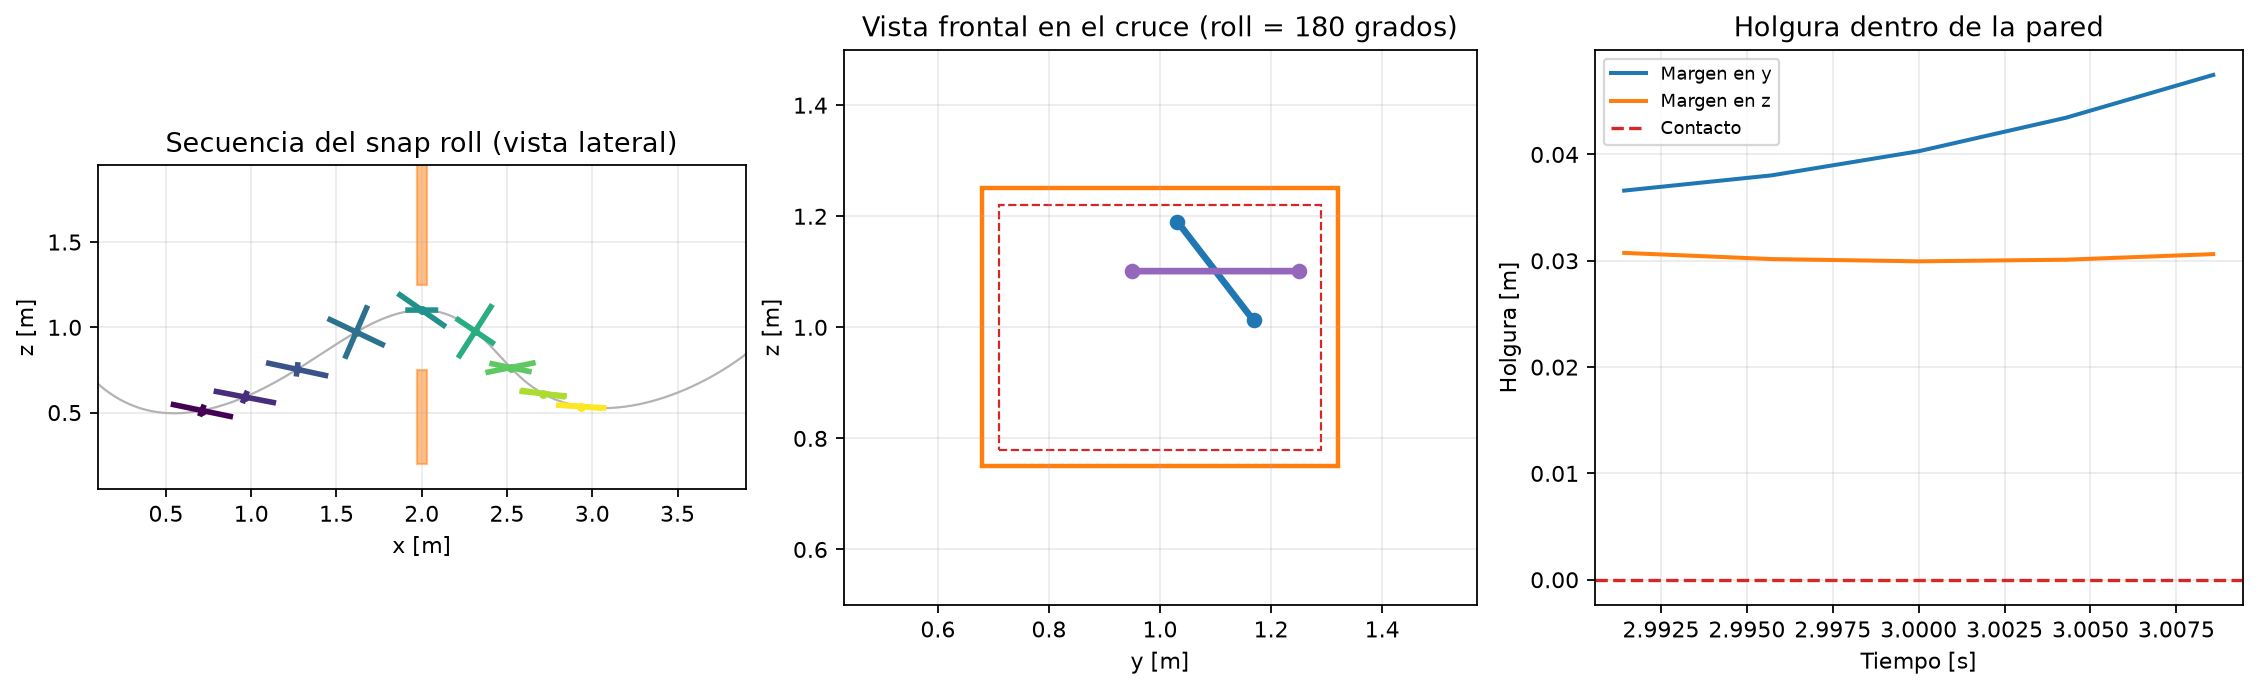
\includegraphics[width=0.95\linewidth]{p2_snap_roll_secuencia.png}
\caption{Secuencia del \textit{snap roll} (vista lateral), vista frontal en el cruce con $\phi=180^\circ$ y holguras de las puntas respecto del borde del agujero.}
\label{fig:p2_sec}
\end{figure}

\subsection{Problema de control óptimo}
\begin{equation*}
\begin{aligned}
\min_{\bx(\cdot),\bu(\cdot)}\quad & J=\int_0^T \ell_c(\bx,\bu)\,dt\\
\text{s.a.}\quad & \dot\bx=\bm f(\bx,\bu),\\
& \bx(0)=\bx_0,\\
& \bx(T)=\bx_f=[\bp_f,\,(2\pi,0,\tfrac{\pi}{2}),\,\mathbf 0],\\
& \\
& 0\le F\le 2mg,\\
& \tau_{\min}\le \tau\le \tau_{\max},\\
& z_{\min}\le z\le z_{\max},\\
& \phi_{\min}\le\phi\le\phi_{\max},\\
& \phi(t_c)=\pi,\\
& \\
& \text{si }|x-x_w|\le e/2:\\
& \quad \big|(y-y_h)\pm\ell\,\bm b_i\!\cdot\!\mathbf e_2\big|\le a-r_r,\\
& \quad \big|(z-z_h)\pm\ell\,\bm b_i\!\cdot\!\mathbf e_3\big|\le b-r_r,\ \ i=1,2.
\end{aligned}
\end{equation*}

Los valores usados son $T=6$\,s, $\tau_{\max}=1$\,N\,m, $\theta_{\max}=0.55$\,rad ($\approx31.5^\circ$), $z\in[0.30,3.20]$\,m y $\phi\in[-0.55,\,2\pi+0.55]$\,rad, de modo que el roll queda libre en $[0,2\pi]$ sin permitir vueltas adicionales. El instante de cruce es $t_c=T/2=3$\,s.

\subsection{Discretización por \textit{multiple shooting}}
Con $N=70$ intervalos, $h=T/N$, $t_k=kh$ y $k_c=N/2$, las variables de decisión son $\bx_1,\dots,\bx_N$ y $\bu_0,\dots,\bu_{N-1}$ ($12N+4N=16N=1120$ variables). El control es constante en cada intervalo y la dinámica se impone con RK4 de dos subpasos de $h/2$ como propagador $\Phi_h$:
\begin{equation*}
\bx_{k+1}-\Phi_h(\bx_k,\bu_k)=\mathbf 0,\qquad k=0,\dots,N-1,
\end{equation*}
lo que da $12N=840$ igualdades, más $12$ igualdades terminales $\bx_N=\bx_f$ y la igualdad $\phi_{k_c}=\pi$. Las restricciones en el cruce son
\begin{align*}
\phi_{k_c}&=\pi,\\
x_{k_c}&=x_w,\\
v_{x,k_c}&\ge v_{c}^{\min},\\
x_{k_c-1}&\le x_w-\tfrac e2,\\
x_{k_c+1}&\ge x_w+\tfrac e2,
\end{align*}

con $v_c^{\min}=2.4$\,m/s. Los dos nodos extremos garantizan que el vehículo entra por un lado de la pared y sale por el otro. La restricción de agujero,
\begin{align*}
\Big|(y-y_h)\pm\ell\,\bm b_i\!\cdot\!\mathbf e_2\Big|\le a-r_r-\delta,\\
\Big|(z-z_h)\pm\ell\,\bm b_i\!\cdot\!\mathbf e_3\Big|\le b-r_r-\delta,
\end{align*}
con margen de seguridad $\delta=0.03$\,m, se impone en tres puntos muestreados del cruce: el punto medio del intervalo $k_c-1$, el nodo $k_c$ y el punto medio del intervalo $k_c$. Las cotas de $z$, $\phi$ y $\theta$ se imponen en nodos y puntos medios. Estas restricciones son suaves, por lo que IPOPT puede derivarlas; como se evalúan en puntos muestreados, no garantizan el no contacto en todo instante continuo, y por ello se verifica después con una simulación fina.

\subsection{Funcional de costo y referencias}
El costo sigue referencias suaves. La posición de referencia $\bp_{\mathrm{ref}}$ es una cúbica de Hermite por tramos que pasa por $\bm c_h$ en $t_c$ con velocidad $(v_c,0,0)$, $v_c=3$\,m/s; el roll de referencia es una vuelta completa en $t_{\mathrm{vuelta}}=1$\,s centrada en $t_c$ y el yaw de referencia gira de $0$ a $\pi/2$ \emph{después} de cruzar:
\begin{align*}
\phi_{\mathrm{ref}}(t)&=2\pi\,s\!\left(\frac{t-(t_c-t_{\mathrm{vuelta}}/2)}{t_{\mathrm{vuelta}}}\right),\\
\psi_{\mathrm{ref}}(t)&=\frac{\pi}{2}\,s\!\left(\frac{t-t_c}{T-t_c}\right),
\end{align*}
con $s(\tau)=10\tau^3-15\tau^4+6\tau^5$ saturada en $[0,1]$. El costo discreto es
\begin{multline*}
J=\sum_{k=0}^{N-1}h\Big[2\|\bp_k-\bp_{\mathrm{ref},k}\|^2+0.02\|\bv_k\|^2+0.5\,\theta_k^2\\
+0.05(\phi_k-\phi_{\mathrm{ref},k})^2+0.12(\psi_k-\psi_{\mathrm{ref},k})^2+0.035\|\bomega_k\|^2\\
+0.025(F_k-mg)^2+0.25\|\btau_k\|^2\Big]+0.02\sum_{k=1}^{N-1}\|\bu_k-\bu_{k-1}\|^2 .
\end{multline*}

\subsection{Inicialización y verificación}
El NLP es no convexo. Como estimación inicial se emplea la referencia que pasa por el centro del agujero; las velocidades se obtienen derivando numéricamente la posición, el cabeceo inicial se estima como $\theta\approx(\cos\psi\,\ddot x+\sin\psi\,\ddot y)/g$, el empuje como $F\approx m(g+\ddot z)$ y los momentos se inicializan en cero. Esta propuesta solo inicializa IPOPT: la solución final la determinan la dinámica, las restricciones y el costo.

Para evaluar la fidelidad respecto del modelo continuo, se integra nuevamente desde $\bx_0$ con DOP853 manteniendo cada $\bu_k$ constante, y se calculan: los defectos de continuidad, la diferencia entre nodos del NLP y la simulación, el error terminal, y el margen $\mathrm{marg}=\min_{i,\pm}\big(\text{semitamaño efectivo}-|\cdot|\big)$ de las cuatro puntas respecto del borde del agujero mientras el vehículo está dentro de la losa. Un margen positivo implica ausencia de contacto.

\begin{figure}[h]
\centering
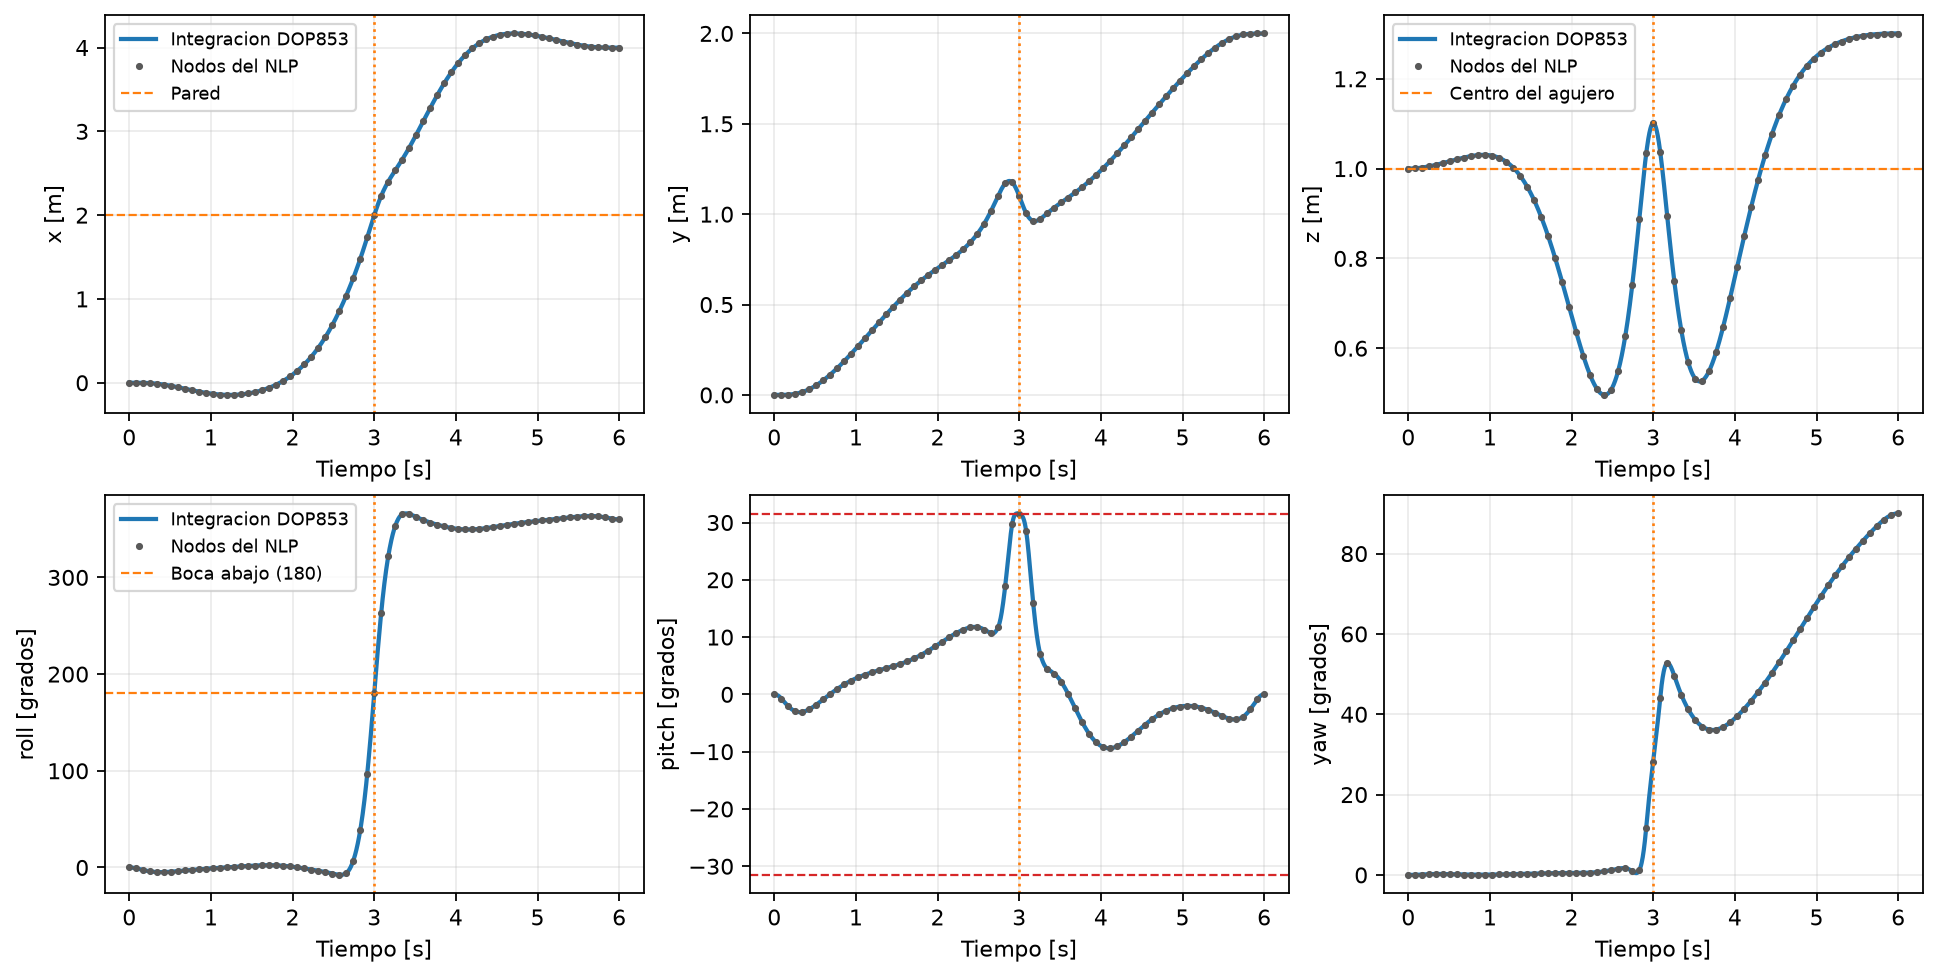
\includegraphics[width=0.85\linewidth]{p2_estados.png}
\caption{Posición y ángulos de Euler. Puntos: nodos del NLP; línea: integración DOP853. La línea punteada vertical marca el cruce ($t_c=3$\,s).}
\label{fig:p2_estados}
\end{figure}

\subsection{Resultados}
La Fig.~\ref{fig:p2_tray} muestra la trayectoria resultante frente a la recta nominal: el vehículo desciende, asciende hasta alinearse con el agujero a $z\approx1.1$\,m, lo cruza en $t=3$\,s con $\phi=180^\circ$ (boca abajo) y luego se estabiliza en $\bp_f$. La Fig.~\ref{fig:p2_estados} compara los nodos del NLP con la integración continua; el roll pasa de $0$ a $360^\circ$ en una ventana corta alrededor del cruce, el yaw alcanza $90^\circ$ al final y el cabeceo llega al límite de $\approx31.5^\circ$ justo en el cruce. Los controles (Fig.~\ref{fig:p2_controles}) muestran el impulso de empuje antes y después del cruce (máximo $\approx15$\,N, por debajo de $2mg\approx19.6$\,N) y saturación de $\tau_x$ en $\pm1$\,N\,m, que es el momento necesario para ejecutar el giro rápido de roll. 

\begin{figure}[h]
\centering
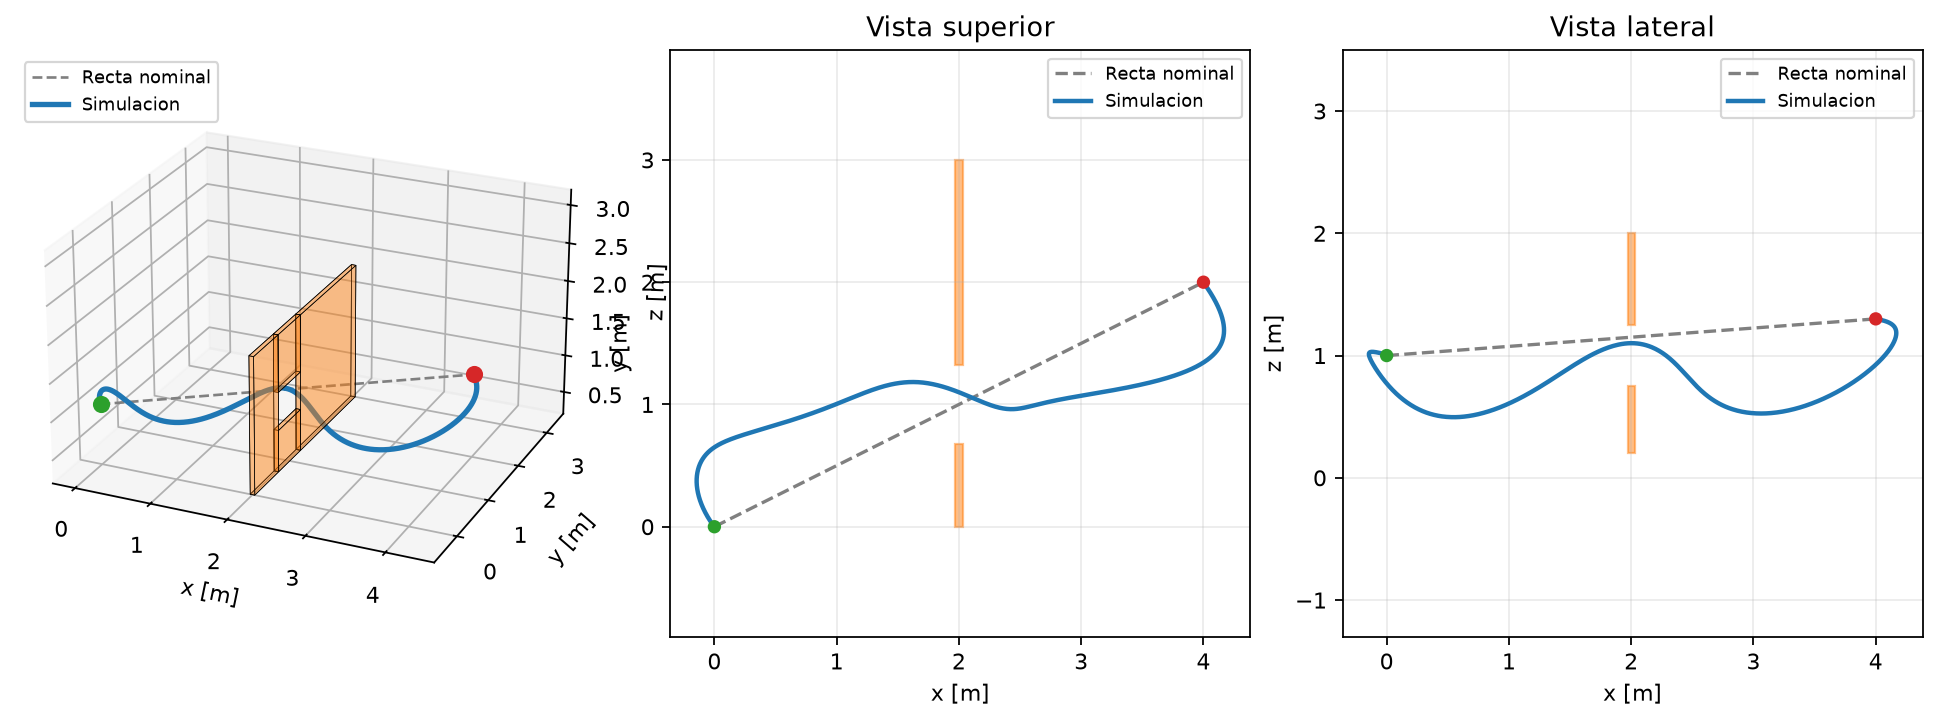
\includegraphics[width=0.85\linewidth]{p2_trayectoria.png}
\caption{Trayectoria 3D, vista superior y lateral frente a la recta nominal.}
\label{fig:p2_tray}
\end{figure}

Finalmente, la Fig.~\ref{fig:p2_sec} muestra la secuencia del \textit{snap roll}, la vista frontal en el cruce y las holguras: las puntas de los rotores permanecen dentro del agujero con márgenes mínimos positivos de $\approx0.03$\,m en $z$ y $\approx0.037$\,m en $y$ mientras el vehículo está dentro de la losa, es decir, sin contacto.

\begin{figure}[h]
\centering
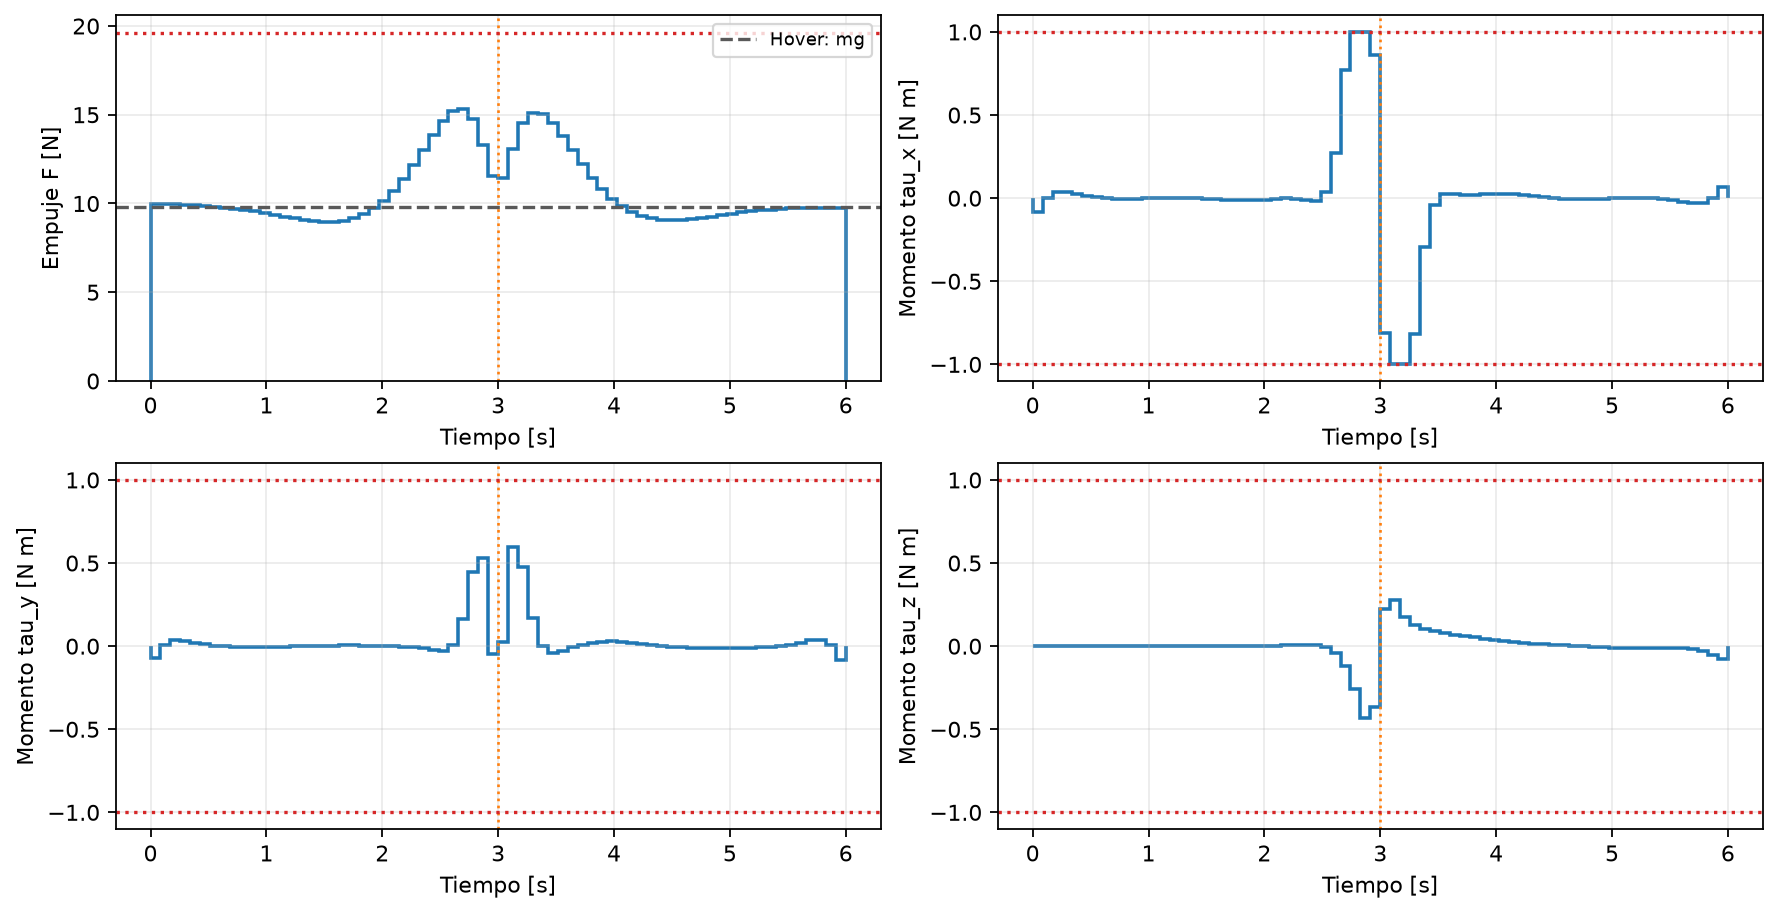
\includegraphics[width=0.85\linewidth]{p2_controles.png}
\caption{Controles óptimos.}
\label{fig:p2_controles}
\end{figure}

\textbf{Animación.} Se adjunta \texttt{p2\_snap\_roll.gif}. El punto rojo marca el extremo delantero del brazo $x$.